%! Author = Ian
%! Date = 12/4/2023

% Preamble
\documentclass[11pt]{article}

% Packages
\usepackage{amsmath}
\usepackage{graphics}
\usepackage{graphicx}

\title{Assignment 5 Writeup}
\author{Ian Chen}
\date{\today}

% Document
\begin{document}
    \maketitle


    \section{Face Detection}

    \begin{itemize}
        \item \textit{Face Classification}\newline
        I used the Viola-Jones algorithm, which uses AdaBoosting to train a strong classifier from a
        subset of Haar-like features. The algorithm is able to achieve a high detection rate while
        minimizing the number of false positives. I generated faces using the FDDB dataset with
        their included bounding boxes.\newline
        I scaled the faces to 24x24 pixels, and the areas of the image not covered by the face were
        deemed non-face regions. I generated the integral images of the training set and its
        corresponding haar-like features. I then used a subset of these features to train the
        boosting algorithm.\newline
        Top classifiers: Decision Stump: (parity=-1, feature\_index=307, threshold=1212
        .2045312499986, error=0.2754251247073025, alpha=-0.96726929195333)\newline
        Decision Stump: (parity=-1, feature\_index=701, threshold=87.74951562500792, error=0
        .29285768037256815, alpha=-0.8815451878903284)\newline
        Decision Stump: (parity=1, feature\_index=402, threshold=-175.16371425779653, error=0
        .3254346857998712, alpha=-0.728906721017052)\newline
        \begin{center}
            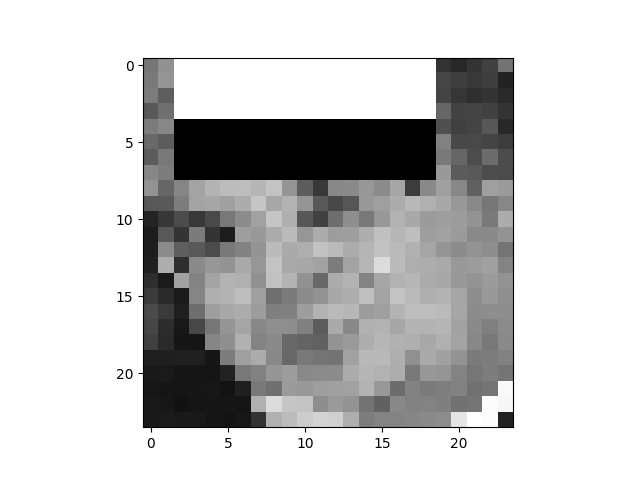
\includegraphics[width=0.3\textwidth]{Output Pictures/rec_1}
            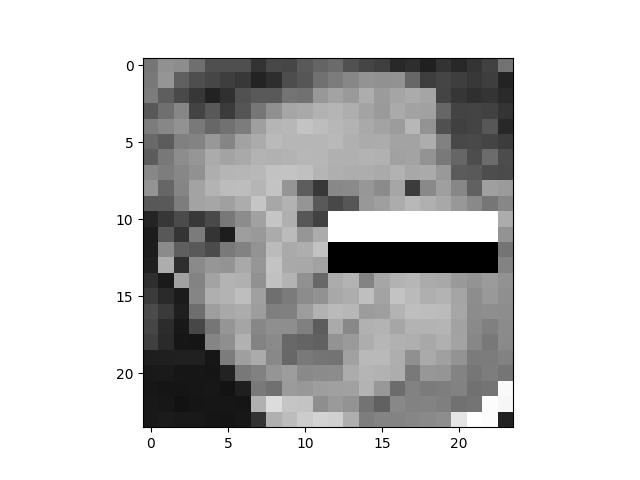
\includegraphics[width=0.3\textwidth]{Output Pictures/rec_2}
            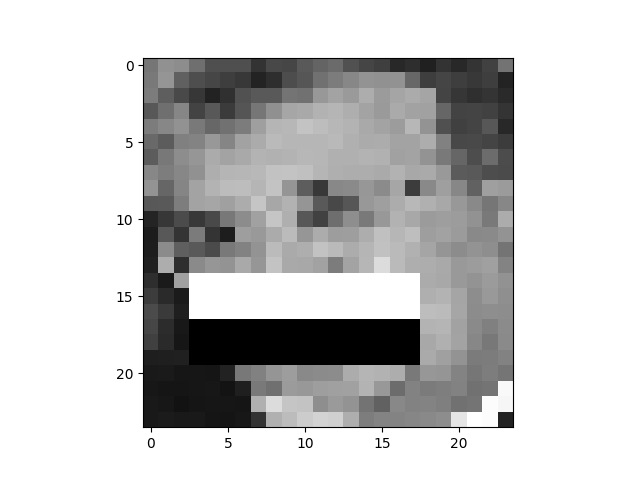
\includegraphics[width=0.3\textwidth]{Output Pictures/rec_3}
        \end{center}

        \item \textit{Sliding Window + Human Classification}\newline
        I used the Viola-Jones algorithm along with the classifier cascade. The algorithm is also
        able to run in real time, as I used the classifier cascade to quickly reject non-face
        regions. Each window has minimal overlap due to my scale factor and step size for the
        cascade. Since every classifier in the cascade has to pass in order for the window to be
        classified as a face, I reduced the threshold of each classifier in the cascade to allow
        more windows to pass through each stage, reducing false negatives. I did this by using my
        trained strong classifier and creating a copy with reduced thresholds.\newline
        \begin{center}
            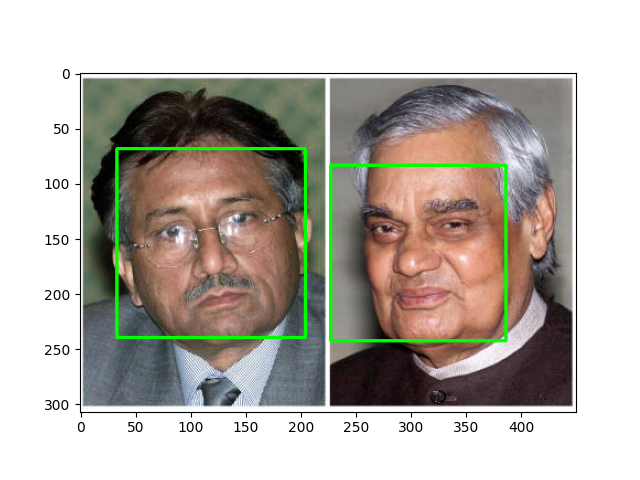
\includegraphics[width=0.3\textwidth]{Output Pictures/ex_1}
            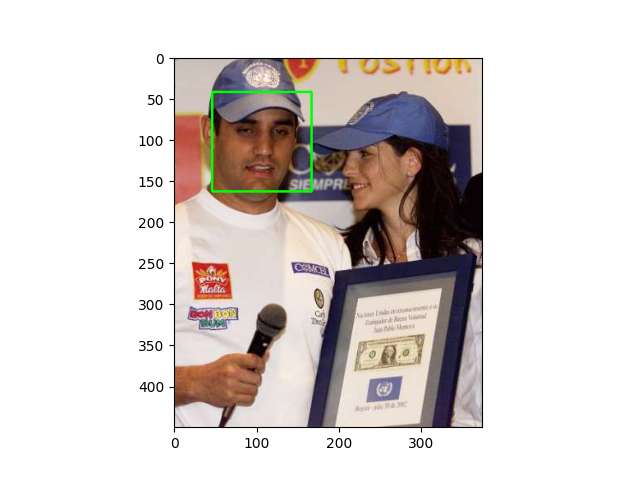
\includegraphics[width=0.3\textwidth]{Output Pictures/ex_2}
            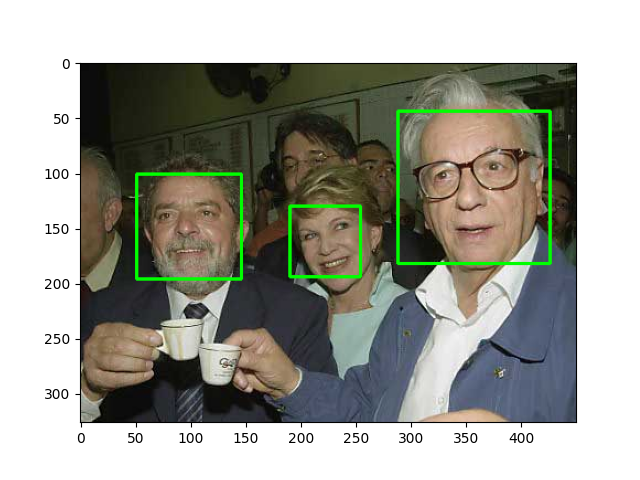
\includegraphics[width=0.3\textwidth]{Output Pictures/ex_3}
        \end{center}
        The algorithm is able to detect faces in the images, but with the classifier cascade, it
        needs fine-tuning to reduce the number of false positives while maintaining a high detection
        rate.\newline
        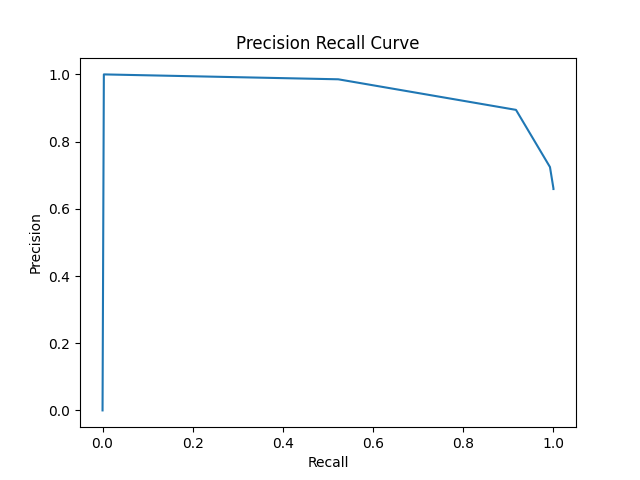
\includegraphics[width=0.3\textwidth]{Output Pictures/prc}

    \end{itemize}


    \section{Extra Credit}

    \begin{itemize}
        \item \textit{Object Detection}\newline
        With the bias using the manhattan distance(L1 Norm) to the average face, the precision
        -recall drop-off is delayed and more gradual. This idea is not computationally expensive
        , and can be used in conjunction with the Viola-Jones algorithm to further reduce the
        number of false positives/negatives.\newline
        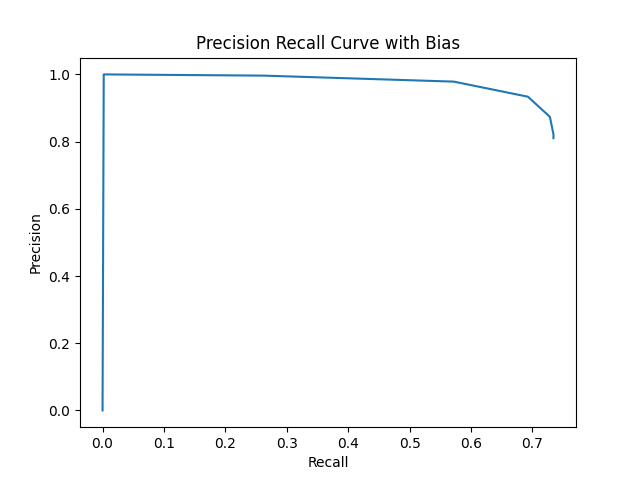
\includegraphics[width=0.5\textwidth]{Output Pictures/prc_knn}

        \item \textit{Running Time}\newline
        Took about 2 and a half minutes to train the classifier, and about 1.5 seconds to test
        the on the provided folds and images. This is assuming all integral images, haar-like
        features, and their corresponding indices are precomputed and cached.\newline
        \begin{center}
            
\includegraphics[width=0.3\textwidth]{Output Pictures/training_start}
            
\includegraphics[width=0.3\textwidth]{Output Pictures/training_finish}
        \end{center}
        \begin{center}
            
\includegraphics[width=0.5\textwidth]{Output Pictures/testing_time}
        \end{center}

        \item \textit{Creative Ideas}\newline
        Unsure if this was explicitly explained in class or the instructions, but I used the
        classifier cascade to quickly reject non-face regions. This greatly increases the speed
        of the algorithm, but it was mentioned in the Viola-Jones paper, which I closely followed
        . One idea I had was to incorporate a KNN-like approach, where I calculated the distance
        of the target image from the average of the faces and non-faces. Shown below.\newline
        \begin{center}
            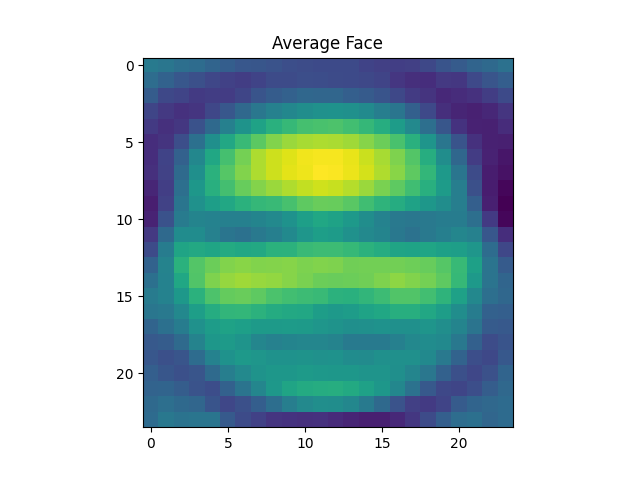
\includegraphics[width=0.4\textwidth]{Output Pictures/average_test_face}
            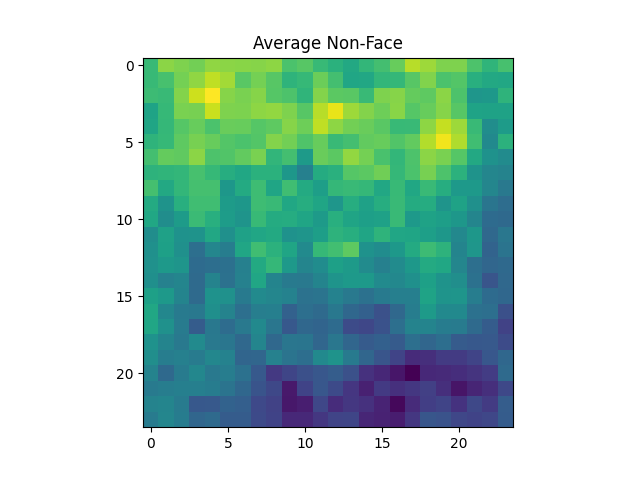
\includegraphics[width=0.4\textwidth]{Output Pictures/average_test_non_face}
        \end{center}

    \end{itemize}
\end{document}